% Packages
\documentclass[11pt,a4paper]{article}
\usepackage[utf8]{inputenc}
\usepackage[T1]{fontenc}
\usepackage{hyperref}
\usepackage{lmodern}
\usepackage[english]{babel}
\usepackage{appendix}
\usepackage{enumitem}

%Fusionneer des pages
\usepackage{pgfpages}
%\pgfpagesuselayout{4 on 1}[a4paper,border shrink=5mm]

% Taille marges
\usepackage[left=2cm,right=2cm,top=2cm,bottom=2cm]{geometry}
% Titles size
\usepackage{titlesec}

% math
\usepackage{amsfonts}
\usepackage{amsmath}
\usepackage{amssymb}
\usepackage{mathabx}
\usepackage{stmaryrd}

\usepackage[most]{tcolorbox}
\newtcolorbox[auto counter]{definition}[1]{colframe=red!75!black, coltitle=white, enhanced, frame empty, colback=white,fonttitle=\bfseries , title=Def \thetcbcounter$\;$: #1, borderline west={2pt}{0pt}{red!85!black},
attach boxed title to top left={xshift=-5mm}, boxed title style={colback=red!75!black}}

\newtcolorbox[auto counter]{prop}{colframe=black!80!white, coltitle=black, enhanced, frame empty, colback=white,fonttitle=\bfseries , title=\underline{Property \thetcbcounter$\;$:}, borderline west={2pt}{0pt}{black},
attach boxed title to top left={xshift=-4mm}, boxed title style={frame empty,colback=white}}

\newtcolorbox[auto counter]{thm}[1]{colframe=blue!70!black,colback=white,fonttitle=\bfseries , title=Theorem \thetcbcounter$\;$: #1}

\newtcolorbox[auto counter]{exercice}{colframe=white,colback=white,fonttitle=\bfseries , title=Exercice \thetcbcounter$\;$:}

\newtcolorbox{preuve}{boxrule=0pt, enhanced, colback=white, colframe=white, coltitle=black, fonttitle=\bfseries , title=\underline{Proof $\;$:},
top=0mm, frame empty, borderline west={1pt}{0pt}{black}, sharp corners,
after upper={\par\hfill\textit{$\blacksquare $}}}

\newtcolorbox{mybox}{colframe=white!75!black,colback=white!95!black,fonttitle=\bfseries}

% pseudo code
\usepackage[ruled,lined,noend]{algorithm2e}
\usepackage{babel}

% insertion image
\usepackage{graphicx}
\graphicspath{ {./images/} }

% derivation tree
\usepackage{ebproof}

% automate
\usepackage{caption}
\usepackage{tikz}
\usetikzlibrary{automata, positioning, arrows, decorations.pathreplacing, decorations.markings, positioning, shapes, quotes}


\newcounter{fig}
\newcommand{\fig}[3]{
	\begin{center}
	\begin{figure}[ht]
		\refstepcounter{fig}
		\centering
		\begin{tikzpicture}[scale=#3]
		#1
		\end{tikzpicture}
		\caption{\underline{#2}}
	\end{figure}
	\end{center}
}

\newcommand{\tab}{\phantom{xxx}}

\newcommand{\ignore}[1]{}

\newcommand{\uao}[3]{\underset{#1}{\overset{#2}{#3}}}

\renewcommand{\lim}[2]{\underset{#1 \rightarrow #2}{lim}}

\newcommand{\mlist}[1]{\begin{itemize}[noitemsep,topsep=0pt]#1\end{itemize}}



\title{\huge{\vspace{-1.0cm}Performance Evaluation project:\\\underline{Optimizing cars' trajectory with AI}}}
\date{}
\author{\vspace{-1cm}Ottavy Macéo, Longatte Mathieu, Mocq Louison}

\begin{document}
\maketitle
%\tableofcontents
\titleformat*{\section}{\huge\bfseries}
\titleformat*{\subsection}{\Large\bfseries}


	\section*{Abstract}

The goal of this project is divided into five parts:
\mlist{
\item Creating a racing car environment to simulate a simple 2D racing car model.
\item Implementing Deep Q-Learning and Genetic Algorithms to optimize the behavior of a car on tracks, enabling it to follow the best possible trajectories.
\item Evaluating the performance of Deep Q-Learning and Genetic Algorithms and comparing their results.
\item Assessing the performance of Deep Q-Learning with respect to different hyperparameters.
\item Evaluating the performance of the best car behavior achieved by both algorithms.
}
You can see the complete project on our public \href{https://github.com/GeckSpy/EP-trajectory-optimisation}{github page}.
% All the code has been developed in Python.

	\section*{Introduction}
	motivation

	\section*{Modeling}
		\subsection*{Racing environment}
			\subsubsection*{Tracks}
A track is originally a .png file wich look like the left image of figure \ref{figure:track}. Then, the image is converted to a matrix $T$ such that $T[0][0]$ is the bottom left corner. After that, we crop the image, compute the starting point and the lines of track (that will be explained in the reward part) to have a final result which look the right image of figure \ref{figure:track}. The white case represent the road, the green point represent the starting point.
\begin{center}
\label{figure:track}
	\begin{figure}[ht]
		\refstepcounter{fig}
		\centering
		
\includegraphics[width=5cm, height=4cm]{track_06.png}
		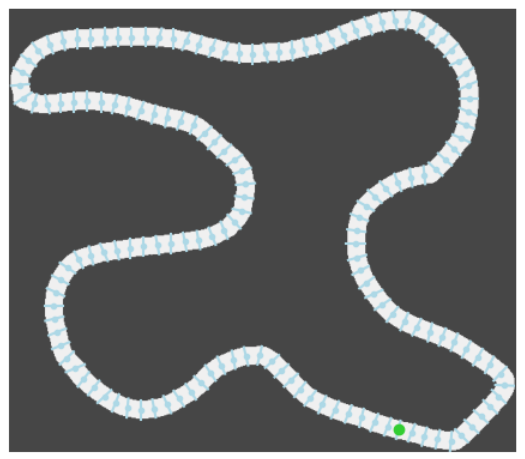
\includegraphics[width=5cm, height=4cm]{track_06_computed.png}
		\caption{\underline{.png and computed track}}
	\end{figure}
\end{center}

	
			\subsubsection*{Cars' physics}
The Car physic is really simple. It is a 2D cartoon-like physics that act as follow:\\
The car has two main informations: its speed $\in [0,$ MaxSpeed$]$ and its rotation $\in [0,360]$. The physics acts as follow: at each times step the car move to next coordinates on the direction of the car's rotation and of distance equal to the car's speed.\\
If the coordinates of the car is $(x,y)$, its speed is $s$ and its rotation is $\alpha$, then, after a time step, the coordinate of the car will be:
\[(s.cos(\frac{\pi}{180}\alpha) + x,\; s.sin(\frac{\pi}{180}\alpha) + y)\]
\\
Moreover, at each time step, the car can make some actions:
\mlist{
\item It can accelerate, this will increase the car's speed by a constant.
\item It can brake, this will decrease the car's speed by reduce the car speed by a constant. The car cannot have a negative speed.
\item It can turn, i.e. add a constant $\in \llbracket-K,K\rrbracket$ to its rotation. $K$ is a constant that is the maximum angle the car can turn per each time step.
}
The behaviour of the car will need to interact with the track therefore we need to decide what is the state of a car, i.e. how the car see the environment. We could give to our algorithms the track matrices and the informations of the car but this will leed to to many parameters because a track can have size $900\times600$. Therefore we will need to train on all possible state wich will be at least $2^{900\times 600}$. Therefore, we decided to give a more realistic state wich represent how a car racer see. Then the state of a car is a array $T$ of size $8$.
\mlist{
\item $T_0$ is the current speed of the car
\item $\forall i\in\{1,...,7\}$, $T_i$ is the distance of the car to the next wall in the direction $\alpha + A_{i-1}$ where $\alpha$ is the current rotation of the car and $A=[60, 40, 20, 0, -20, -40, -60]$
}
Then, the representation looks like figure \ref{figure:car state}.
\begin{center}
\label{figure:car state}
	\begin{figure}[ht]
		\refstepcounter{fig}
		\centering
		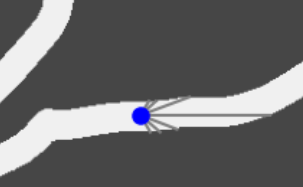
\includegraphics[width=4cm, height=3cm]{car_state.png}
		\caption{\underline{Car state}}
	\end{figure}
\end{center}
		
			\subsubsection*{Technical aspects of the environment}
To manipulate our environment, we use the python packages \texttt{gymnasium} which provide code convention for those type or environment, i.e. environment where at each time step, you have one action to do. The environment has to have some essential function: \texttt{reset()} that reset the environment to be able to do an other simulation, \texttt{render()} that render the current state of our environment and the most important one is \texttt{step()} that do one step of time, i.e. given an action, the \texttt{step()} function figure out is the car has crashed or not, move the car to its next position and return the new state of the car, a reward and if the car has crashed.\\
Our environment has a variable named \texttt{time} which give us the opportunities to discreet more or less the time.
		
			\subsubsection*{Rewards}
For those type of problem where the AI model has to compute a behavior, the AI model produces something which look like a function $f$ that take a car state and return an action. We need to specifies to our AI model when it produce a good action and a bad action, for instance, if a car crash, we need to punish the AI model.\\
We do that thanks to a function reward implemented in the function \texttt{step()} of our environment. The reward is an integer, the bigger it is the best the action was. The function might be the most important one of all the project because it is thanks to it that our AI model will perform well or not. We try lot of reward function and we finish by using the following one. To punished the car when it do something bad we do:
\mlist{
\item If the car crashes, we stop the simulation and return a reward of $-500$
\item If the car is not moving, i.e. has a speed of $0$, the reward is $-10$
}
For the positive reward, we have automatically computed some track line (represented in right image of figure \ref{figure:track}). If the car crosses next line, it has a reward of $(+10\times$ the number of lines it has cross in the good order with this action). If the car cross a line in the wrong order, it means that it has gone backward, therefore, we punished the car with a reward of $-200$ and we stop the computation.\\
On top of that, at each time step, we add to the current reward the speed of the car divided by a constant to encourage the car to go fast.

			\subsubsection*{Conclusion}
After explaining all of this, here is an example in figure \ref{figure:env example}. We have plot the trajectory of the car, the green color is when the car has accelerate, red color when it brake and yellow otherwise.
\begin{center}
\label{figure:env example}
	\begin{figure}[ht]
		\refstepcounter{fig}
		\centering
		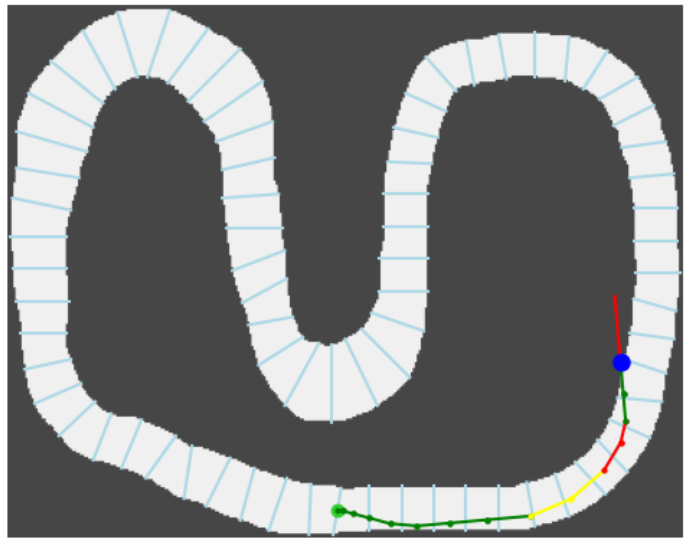
\includegraphics[width=6cm, height=5cm]{env_example.png}\\
		List of rounded reward: \texttt{[10, 1, 2, 12, 13, 13, 13, 14, 24, 14, 13, 12, 13, -497]}
		\caption{\underline{Car state}}
	\end{figure}
\end{center}
The total reward of a car behaviour is the sum of all reward of a simulation with a car behaviour. For example, the reward of the car behaviour or the figure \ref{figure:env example} is $-343$.


		\subsection*{Deep Q-learning}
Deep Q-Learning is a reinforcement learning algorithm that combines Q-Learning with Deep Learning to solve complex decision-making problems. It allows an agent to learn how to act optimally in environments with large state spaces by approximating a function, known as the \textit{Q-function}, which evaluates the quality of an action taken in a given state.
    
            \subsubsection*{Q-function}
The Q-function, $Q(s, a)$, represents the expected cumulative reward an agent will receive after taking action $a$ in state $s$, and then following the optimal policy. The cumulative reward is computed as:
\[Q(s, a) = r + \gamma \max_{a'} Q(s', a'),\]
Where:
\mlist{
\item $r$ is the immediate reward received after taking action $a$ in state $s$.
\item $s'$ is the next state reached.
\item $a'$ is the next action.
\item $\gamma \in [0, 1]$ is the discount factor, which balances immediate and future rewards.
}
% \subsection*{Deep Q-Learning}
% In DQL, a deep neural network, called the \textit{Q-network}, is used to approximate the Q-function. This network takes the state $s$ as input and outputs estimated Q-values for all possible actions. By doing so, DQL can handle environments with high-dimensional or continuous state spaces.
    
            \subsubsection*{Key Techniques}
\mlist{
    \item \textbf{Replay Buffer}: A memory that stores past experiences $(s, a, r, s')$. Randomly sampling experiences from the buffer during training reduces correlations between consecutive samples, improving learning stability.
    \item \textbf{Exploration-Exploitation Balance}: The agent uses an $\epsilon$-greedy policy to choose actions, where it explores randomly with probability $\epsilon$ and exploits the best-known action otherwise.
}
    
            \subsubsection*{High-Level Workflow}
\mlist{
\item Observe the current state $s$.
\item Choose an action $a$ using an $\epsilon$-greedy policy.
\item Execute the action, observe the reward $r$ and next state $s'$.
\item Store the experience $(s, a, r, s')$ in the replay buffer.
\item Sample a mini-batch of experiences from the buffer to train the Q-network.
}
    


	
		\subsection*{Genetic algorithms}
			\subsubsection*{What are genetic algorithms?}
Genetic algorithms (GA) are probabilistic algorithms based on natural selection. Therefore, GA takes some populations which are sets of solutions (here a solution is a car's behaviour), select the best solutions thanks to the reward function. Then, it changes the population by adding new random solutions, adding some mutations which are some small variations of a behaviour, adding some cross-over which are the equivalent of natural reproduction. We can either repeat this process a fixed number of generations or for a fixed amount of time.
		
			\subsubsection*{Markov Chain modelisation}
We will now introduce a Markov chain modelisation to genetic algorithm. We define a Markov chain $(Y_n)_{n\in\mathbb{N}}$ as following:
\mlist{
\item A state of $(Y_n)_{n\in\mathbb{N}}$ is a population.
\item Let $y_0$ be a special state such that if $Y_n = y_0$ then it means that the population of state $Y_n$ contain an optimal solution.
}
\tab \\
Now, the sequence of population of genetic algorithm can be describe with this Markov chains. $Y_n$ represent the population at generation $n$. Notice that the state $y_0$ is an absorbing state. In fact if $Y_n = y_0$ then it mean that the population $P_n$ contain an optimal solution. Since we always keep the best solution of the previous population, it means that $\forall n'>n$, we have that $P_{n'}$ contain an optimal solution. Therefore, $\forall n'>n$, $Y_{n'} = y_0$. Moreover, $y_0$ is the only absorbing state of $(Y_n)_{n\in\mathbb{N}}$.\\
\\
If we suppose that our mutation and cross-over are made such that a solution $x$ can reach $y$ by a series of a finite number of those operations. Then, all solutions $x$ can reach an optimal value. Then every state $y_n$ can reach state $y_0$. The set of all possible state is finite. Then $\mathbb{P}(Y_n = y_0) \underset{n \rightarrow +\infty}{\rightarrow} 1$\\
Then $\mathbb{P}($ The population $P_n$ contain an optimal solution$) \underset{n \rightarrow +\infty}{\rightarrow} 1$\\
Thus, the genetic algorithm converge toward a global optimal solution. However, we do not know how many time it will take in average.
		
			\subsubsection*{NEAT}
Basic genetic algorithms are not efficient enough to compute an optimize behavior. Therefore, we will use the famous python packages called \texttt{NEAT}. It is an optimized generalized genetic algorithms with represent solution as dynamic neural network. By dynamic we mean that the algorithm can add or delete some of the nodes of the neural network. The principle of GA stay the same but we have a lot more hyper parameters.
	
	
	\section*{Simulation}
Once we completed the modeling of the environment, the deep Q-learning algorithm and the genetic algorithm, we have to compute some simulation to process evaluation performance. We will compare our two algorithm using various metrics. For this purpose, we choose the following metric: the average reward after training depending of some parameter. We measure this value across different training durations and varying the numbers of tracks used to training the models. To ensure robustness and evaluate potential over-fitting, we test the models on tracks that were not included in the training set.\\
This approach is applied in the context of an AI project where we train AI agents to complete a racing circuit. The goal is for the cars to complete laps as quickly as possible, and the average reward reflects their performance under these conditions. We used \textbf{grid5000} to train our model. First for research reproducibility, to have stable computer and to have access to strong GPUs.
\mlist{
\item First, we will compare genetic algorithm to Q-learning depending of the training time and the number of track used to train the car. We we train our algorithms during 10 to 60 minutes and with 10 to 67 tracks.
\item Then, we compare the result of deep Q-learning depending of some hyper-parameters.
\item Finally, we will evaluate the performance or the best car we found using deep Q-learning with a training of six hours.
}

    \section*{Experimental}
DES BEAUX PLOT LOUISON JE T'EN SUPPLIE

		\subsection*{Comparing Genetic Algorithm and Deep Q-Learning }
metrics: GA VS Q: training time : 10, 40, 60, number of tracks: 10, 40, 0.8 times number of tracks

		
		\subsection*{Deep Q-Learning Hyper Parameter}
		
		\subsection*{Best Car}

	



    \section*{Conclusion}
	

\end{document}